\documentclass[addpoints,12pt]{exam}
%\usepackage[fontsize=18pt]{scrextend}
\newcommand{\ds}{\displaystyle}
\usepackage[margin=0.8in]{geometry}
\usepackage{subcaption}
\usepackage{pgfplots}
\usepackage{multicol}
\pgfplotsset{compat=1.16}

\usepackage{amssymb,amsmath,graphicx,wrapfig,verbatim, psfragx,color,todonotes}
\usepackage{multicol}
\usepackage{wasysym}
\newcommand*{\Scale}[2][4]{\scalebox{#1}{\ensuremath{#2}}}%

% \usepackage{amssymb,amsmath,graphicx,wrapfig,verbatim, psfragx,color}
% \usepackage{multicol}
% \usepackage{wasysym}
\usepackage{tikz}
\usetikzlibrary{fit}
\usetikzlibrary{shapes}
\usetikzlibrary{calc}
\usetikzlibrary{3d}
\pgfplotsset{my style/.append style={axis x line=middle, axis y line=
middle, xlabel={$x$}, ylabel={$y$}, axis equal }}



% If you want them as a list (instead of next to each other)
\usepackage{enumitem}

% ---- Convenience commands -----

% Choose one option (bubbles)
\newcommand{\chooseone}{{\Large$\Circle$\ \ }}

% ---- Example Usage | Multiple Choice -----


%\usepackage{fancyhdr}
%\setlength{\headheight}{13.6pt}
%\pagestyle{fancy}
%\lhead{Math 222}
%\chead{ Midterm 1 }
%\rhead{Spring 2022}

\def\FillInBlank{\rule{3truein} {.01truein}}
\newcommand{\TorF}{\hspace{.1in} \textbf{True} \hspace{.1in} \textbf{False}  \hspace{.1in}}


\newcommand{\myleft}{\makebox[.4\textwidth]{First Name:\enspace\hrulefill}}
\newcommand{\myright}{\makebox[.4\textwidth]{Last Name:\enspace\hrulefill}}
\header{\oddeven{\myleft}{}}
       {}
       {\oddeven{\myright}{}}

\footrule

\footer{Math 112}
       {Final - 
       Spring 2025}
       %Fall 2024}
       {Page \thepage\ of \numpages}

\begin{document}

Multiple choice section. All points are for choosing the correct answer. No justification is needed.
\begin{questions} 

\question[3] Starting form the base function $|x|$ (graph shown below). 

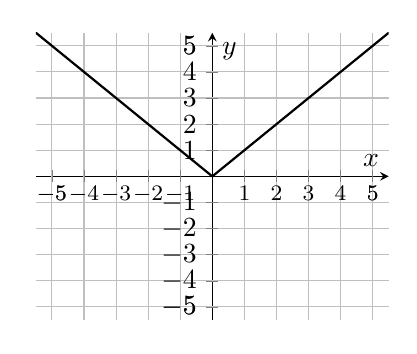
\begin{tikzpicture}
\begin{axis}[
   grid = major,
   extra x ticks={-6,-5,-4,-3,-2,-1,1,2,3,4,5,6},
   extra y ticks={-6,-5,-4,-3,-2,-1,1,2,3,4,5,6},
   %ytick= false,
   %xminorgrids=true,
   width=.5\textwidth,
   %clip = true,
   %clip mode=individual,
   %restrict y to domain=-12:12,
   axis x line = middle,
   axis y line = middle,
   %     yticklabel style = {font=\footnotesize,xshift=0.5ex},
        xticklabel style = {font=\footnotesize,yshift=0.5ex},
   xlabel={$x$},
   %xlabel style={at=(current axis.right of origin)},
   ylabel={$y$},
   %ylabel style={at=(current axis.above origin)},
   %domain = -5:5,
   xmin = -5,
   xmax = 5,
   enlarge y limits={rel=0.05},
   enlarge x limits={rel=0.05},
   ymin = -5,
   ymax = 5,
 ]
\addplot[smooth, thick, domain = -6:0,samples=2
	] { abs(x)};
\addplot[smooth, thick, domain = 0:6,samples=2
	] { abs(x)};
% \addplot[smooth, thick, domain = 1.15:6.5,
%	] { (3*x^2+5*x-2)/(x-1)};
\end{axis}
\end{tikzpicture}

Select the function graphed below. %[Select \textbf{ONE}]

\begin{multicols}{2}
    

    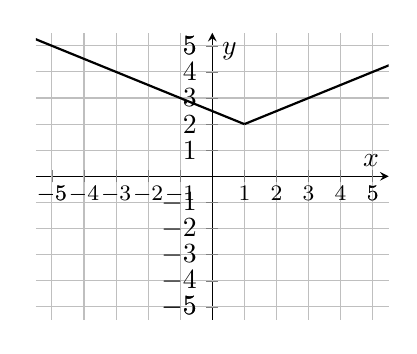
\begin{tikzpicture}
\begin{axis}[
   grid = major,
   extra x ticks={-6,-5,-4,-3,-2,-1,1,2,3,4,5,6},
   extra y ticks={-6,-5,-4,-3,-2,-1,1,2,3,4,5,6},
   %ytick= false,
   %xminorgrids=true,
   width=.5\textwidth,
   %clip = true,
   %clip mode=individual,
   %restrict y to domain=-12:12,
   axis x line = middle,
   axis y line = middle,
   %     yticklabel style = {font=\footnotesize,xshift=0.5ex},
        xticklabel style = {font=\footnotesize,yshift=0.5ex},
   xlabel={$x$},
   %xlabel style={at=(current axis.right of origin)},
   ylabel={$y$},
   %ylabel style={at=(current axis.above origin)},
   %domain = -5:5,
   xmin = -5,
   xmax = 5,
   enlarge y limits={rel=0.05},
   enlarge x limits={rel=0.05},
   ymin = -5,
   ymax = 5,
 ]
\addplot[smooth, thick, domain = -6:1,samples=2
	] { .5*abs(x-1)+2};
    \addplot[smooth, thick, domain = 1:6,samples=2
	] { .5*abs(x-1)+2};
% \addplot[smooth, thick, domain = 1.15:6.5,
%	] { (3*x^2+5*x-2)/(x-1)};
\end{axis}
\end{tikzpicture}
\begin{choices}
    \choice $f(x)=2|x-1|+2$
    \choice $f(x)=2|x+1|+2$
    \choice $f(x)=\frac{1}{2}|x-1|+2$
    \choice $f(x)=\frac{1}{2}|x+1|+2$
    \choice None of the above.
\end{choices}
\end{multicols}

\question[3] Which of the following is a polynomial, $p(x)$ with roots of $-3$, $\sqrt{2}$, and 1.% (which may or not be repeated) and $p(x)\to+\infty$ as $x\to-\infty$
\begin{choices}
   \choice \chooseone $p(x)=(x-3)(x+2)^2(x+1)$
   \choice \chooseone $p(x)=(x+3)(x-2)^2(x-1)$
    \choice \chooseone $p(x)=(x-3)(x+\sqrt{2})(x+1)$
   \choice \chooseone $p(x)=(x+3)(x-\sqrt{2})(x-1)$

   \choice \chooseone None of the above.
\end{choices}

\question[3] 
Consider the parabola $f(x)=(x+3)^2+k$. What is $k$ if $f(x)$ has only one zero?
\begin{choices}
   \choice \chooseone $k=0$
   \choice \chooseone $k>0$
   \choice \chooseone $k=-9$
   \choice \chooseone $k=-3$
   \choice \chooseone None of the above.
\end{choices}

\newpage

\question[3] Consider the rational function 
\[
f(x)=\dfrac{x^3+5x+3}{2x^2+1}
\]
What can we say about any asymptotes for this function?
\begin{choices}
   \choice \chooseone $f(x)$ has a horizontal asymptote at $y=0$.
   \choice \chooseone $f(x)$ has a horizontal asymptote at $y=\dfrac{1}{2}$. 
   \choice \chooseone We cannot say anything about asymptotes of $f(x)$.
      \choice \chooseone $f(x)$ has a slant asymptote.
   \choice \chooseone None of the above.
\end{choices}

\question[3] Let $f(x)=x^2-\sqrt{x+1}$ and $g(x)=\dfrac{-3}{2x}$, what is $f(g(x))$?
\begin{choices}
   \choice \chooseone $\dfrac{-3x}{2}+\dfrac{3\sqrt{x+1}}{2x}$
      \choice \chooseone $\dfrac{9}{4x^2}-\sqrt{\frac{-3}{2x}+1}$
   \choice \chooseone $\dfrac{-9}{4x^2}-\sqrt{\frac{-3}{2x}+1}$

   \choice \chooseone $\dfrac{-3}{2x^2-2\sqrt{x+1}} $
   \choice \chooseone None of the above.
\end{choices}

\question[3] What is the domain of the following function:
\[
f(x)=\dfrac{\sqrt{x+3}}{x-5}
\]
\begin{choices}
   \choice \chooseone $[-3,\infty)$
   \choice \chooseone $(-\infty,5)\bigcup(5,\infty)$
   \choice \chooseone $[-3,5)\bigcup(5,\infty)$
   \choice \chooseone $(-\infty,\infty)$
   \choice \chooseone None of the above.
\end{choices}

\newpage
\hspace{-.5in}Free answer section. \textbf{Work must be shown to get credit for any answer.} Partial credit may be given even for incorrect final answers, so show your work.

% Penny: abs inequality
\question[7] Solve the following inequality and write your answers in interval notation. 
\begin{equation*}
|7x + 3| + 8 \geq 13\,
\end{equation*}
% 1pt: show some understanding
% 1pt: \geq 5 case
% 1pt: correct x\geq 2/7
% 1pt: \leq -5 case
% 1pt: correct x \leq -8/7
% 1pt: interval, brackets

\vfill
\begin{center}
            $
               \mbox{Interval(s)}: \Scale[1.5]{\boxed{ \phantom{\dfrac{a}{b}} \hspace{5cm} }}
            $
            \end{center}
\question[7] Combine the following into a single fraction with no common factors on the top and bottom.

\[
\dfrac{3}{5x^2-10x}+\dfrac{2x}{x-2}
\]
\vfill
\begin{center}
            $
                \mbox{$f(x)=$ } \Scale[1.5]{\boxed{ \phantom{\dfrac{\dfrac{a}{b}}{b}} \hspace{5cm} }}
            $
            \end{center}
\newpage


% Dewei's problem for sec 3.1
\question
\begin{parts}
    \part[6] Write the function $f(x)=2x^{2}+4x+7$ in vertex form, $a(x-h)^2+k$.% and find the coordinates of the vertex. Is the vertex a max or a min?
\vfill\vfill\vfill\vfill
\begin{center}
            $
                \mbox{$f(x)=$ } \Scale[1.5]{\boxed{ \phantom{\dfrac{a}{b}} \hspace{5cm} }}
            $
            \end{center}
    \part[2] What are the coordinates of the vertex?
    \begin{center}
    
            $
                \mbox{Vertex: } \Scale[1.1]{\boxed{ \phantom{\frac{a}{b}} \hspace{4cm} }}
            $ 
    \end{center}
    \part[2] Is the vertex a maximum or a minimum?
    \begin{choices}
   \choice \chooseone Maximum.
   \choice \chooseone Minimum.
\end{choices}
\end{parts}




% %I am not sure how many points should be assigned here; if there are totally 5 points, I would distribute them like this:
% % 1 for any attempt solving this, since this is the final and I don't want to be too harsh to them
% % 2 for completing the square (if they recognized to do so but failed, like computation mistakes or don't know how to do the algebraic transform, give partial points)
% % 1 for the coordinate of the vertex
% % 1 for pointing out this is a max
% % Other attempts for solving the problem should also be accepted.

\question[4]
Write the following as a single log.
\[
f(x)=4\ln(x+2)-\frac{1}{2}\ln z+y\ln 3
\]
\vfill
\begin{center}
            $
                \mbox{$f(x)=$ } \Scale[1.5]{\boxed{ \phantom{\dfrac{\dfrac{a}{b}}{b}} \hspace{5cm} }}
            $
            \end{center}
\newpage

% %Taeyoung's problem for sec 3.3
% \question[8]
% Use a polynomial long division to find the quotient and the remainder of the following polynomial division:

% $$(2x^3-5x^2+2x-15)\div (x+2)$$

% \vfill\vfill\vfill

% %this question has 8 points because I think the following rubric is best: 2 pts for trying to do long division, 3 pts for the correct first step in the long division, 3 pts for the correct second step in the long division.
% %this page should be reserved for this problem as students will need a space to do the long division.
% \question[6]
% Find the real valued solution(s) to the following equation:
% \[
% e^{2x}-3e^x-10=0
% \]
% \vfill
% \begin{center}
%             $
%                 \mbox{$x=$} \Scale[1.5]{\boxed{ \phantom{\dfrac{a}{b}} \hspace{5cm} }}
%             $
%             \end{center}
% \newpage

\question Consider the rational function
\[
f(x)=\dfrac{x-5}{x^2+2x}
\]
\begin{parts}
\part[2] Find the zero(s) of $f$
\vspace{1cm}
\begin{center}
            $
                \mbox{$x=$ } \Scale[1.5]{\boxed{ \phantom{\dfrac{a}{b}} \hspace{5cm} }}
            $
            \end{center}
\part[2] Find the vertical asymptote(s) of $f$
\vspace{1cm}
\begin{center}
            $
                \mbox{$x=$ } \Scale[1.5]{\boxed{ \phantom{\dfrac{a}{b}} \hspace{5cm} }}
            $
            \end{center}
\part[4] For what intervals of $x$ is $f(x)\le 0$
\vfill
\begin{center}
            $
               \mbox{Interval(s)}: \Scale[1.5]{\boxed{ \phantom{\dfrac{a}{b}} \hspace{5cm} }}
            $
            \end{center}
\end{parts}
\question[8] Find the inverse function for the function below:
\[
f(x)=\dfrac{2x}{5-3x}
\]
\vfill
\begin{center}
            $
                \mbox{$f^{-1}(x)=$ } \Scale[1.5]{\boxed{ \phantom{\dfrac{\dfrac{a}{b}}{b}} \hspace{5cm} }}
            $
            \end{center}
\newpage

%alejandro's problem for sec 3.7 polynomial inequality
%---------------CONSENT NOT GRANTED FOR INCLUSION IN FUTURE BASE NOTES--------------------------
%alejandro's problem for sec 4.1-4.2 compound interest
%---------------CONSENT NOT GRANTED FOR INCLUSION IN FUTURE BASE NOTES--------------------------



\question[7]
Solve the following equation for $x:$
    \begin{align*}
        \log_{6}(x)+\log_6 (x-1) = 1
    \end{align*}
\vfill
        \begin{center}
$
                \mbox{$x$ = } \Scale[1.5]{\boxed{ \phantom{\dfrac{a}{b}} \hspace{5cm} }}
            $
%\Huge{\boxed{\phantom{\frac{1}{2}} t = \hspace{9cm} }}
\end{center}
\question[7]
% \begin{parts}
%     \part 
    For what value(s) of $x$ does
    \begin{align*}
        \left(\ln(x)\right)^2 - 3\ln(x)=0\,?
    \end{align*} \vfill
    % \part 
            \begin{center}
$
                \mbox{$x$ = } \Scale[1.5]{\boxed{ \phantom{\dfrac{a}{b}} \hspace{5cm} }}
            $
%\Huge{\boxed{\phantom{\frac{1}{2}} t = \hspace{9cm} }}
\end{center}
    \newpage
    \question A swimming pool is being emptied, and the amount of water (in liters) in the pool at time $t$ (in minutes) is given by 
    \[P(t) = P_0 \cdot 5^{rt}\] where \(P_0\) and \(r\) are some constants. If there is initially $1000$ liters of water in the pool, and after $7$ minutes there is $500$ liters of water in the pool, find the values of $P_0$ and $r$. 
    \begin{parts}
        \part[2] What is $P_0$?
        \vspace{1cm}
        
        \begin{center}
$
                \mbox{$P_0$ = } \Scale[1.5]{\boxed{ \phantom{\dfrac{a}{b}} \hspace{5cm} }}
            $
%\Huge{\boxed{\phantom{\frac{1}{2}} t = \hspace{9cm} }}
\end{center}
        \part[4] What is $r$? (Leave the value for $r$ in terms of a logarithm.)
       \vspace{8cm}
        \begin{center}
$
                \mbox{$r$ = } \Scale[1.5]{\boxed{ \phantom{\dfrac{a}{b}} \hspace{5cm} }}
            $
%\Huge{\boxed{\phantom{\frac{1}{2}} t = \hspace{9cm} }}
\end{center}

\part[2] Knowing that the pool is being emptied, is $r$ positive or negative?
\begin{choices}
   \choice \chooseone $r$ is positive
   \choice \chooseone $r$ is negative
\end{choices}

    \end{parts}
    % \end{parts}
\newpage

%Chenghuang's problem for sec 3.4 and 3.5
\question[8] Consider the following polynomial 
\[ q(x)= 3x^3+16x^2+3x-10\]
Suppose we know $q(x)$ has a root $x=-1$, write $q(x)$ as a product of linear factors.
%this question has 6 points because I think the following rubric is best: 2 pts for knowing x+1 is a factor, 2 pts for the correct long division by x+1, 2 pts for the correct final step. If students choose wrong factor to do long division (like x-1) and try to do long division, give 2 points total.
%Since Taeyoung's problem already has long division, I try to make the long division here as simple as possible.
\vfill

\begin{center}
$
                \mbox{$q(x)$ = } \Scale[1.5]{\boxed{ \phantom{\dfrac{a}{b}} \hspace{5cm} }}
            $
%\Huge{\boxed{\phantom{\frac{1}{2}} t = \hspace{9cm} }}
\end{center}

\newpage
\question[8]
For the following system of linear equations, determine whether or not the system has any solutions. If the system has a solution, state it as an ordered pair $(x,y)$; if the systems has infinitely many solutions, write your solutions as an ordered pair in terms of the variable $x$ only.
$$\begin{cases}
4 x  +  3 y & = 7 \\
- x  +  2 y & = 5
\end{cases}$$
\vfill
\begin{center}
    

$
                (x,y) = \Scale[1.5]{\boxed{ \phantom{\dfrac{a}{b}} \hspace{5cm} }}
            $
            \end{center}

\end{questions}





\end{document}
